\subsection{Octree > Resample}
\label{subsection:resampleWithOctree}

\begin{figure}[!htb]
\begin{center}
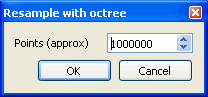
\includegraphics[width=0.25\textwidth]{Partie3_Fonctions/resampleWithOctreeDlg.png}
\caption{\label{fig:resampleWithOctreeDlg}Interface pour r�-�chantillonnage par Octree}
\end{center}
\end{figure}

\index{echantillonner@�chantillonner!re-echantillonner@r�-�chantillonner}
Fonction de r�-�chantillonnage (grossier) d'un nuage. L'utilisateur sp�cifie un nombre approximatif de points (via
l'interface~\ref{fig:resampleWithOctreeDlg}), et \emph{CloudCompare} d�termine alors le niveau d'octree ayant un
nombre de cellules le plus proche de cette valeur. Le nuage r�-�chantillonn� est alors form� en rempla�ant chaque
cellule par un point \emph{repr�sentatif} (actuellement, le centre de gravit� des points pr�sents � l'int�rieur de
la cellule).\\
\par
Remarque : cette m�thode est diff�rente de la m�thode \emph{Subsample} (Cf. section~\ref{subsection:subsample})
car elle cr�e de nouveaux points 3D � des positions diff�rentes de celles des points d'origine, contrairement � la m�thode \emph{Subsample} qui ne fait que s�lectionner des points existants dans le nuage d'origine.
